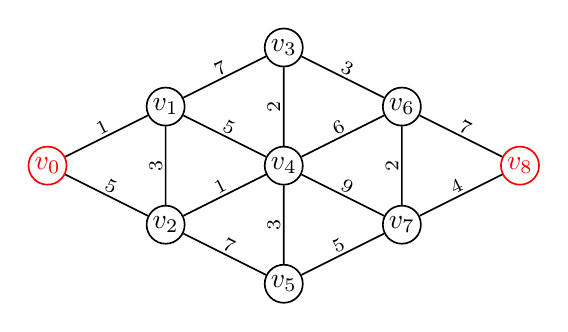
\begin{tikzpicture}[scale=1.5,node distance=1.5cm,semithick,inner sep=1pt,bend angle=45,sloped,anchor=south]
%\draw[help lines] (-3,-3) grid (3,0);
\node[circle,draw,red] (v0)  at(0,0)    {$v_0$};
\node[circle,draw] (v1)  at(1,0.5) {$v_1$};
\node[circle,draw] (v2)  at(1,-0.5) {$v_2$};
\node[circle,draw] (v3)  at(2,1) {$v_3$};
\node[circle,draw] (v4)  at(2,0) {$v_4$};
\node[circle,draw] (v5)  at(2,-1) {$v_5$};
\node[circle,draw] (v6)  at(3,0.5) {$v_6$};
\node[circle,draw] (v7)  at(3,-0.5) {$v_7$};
\node[circle,draw,red] (v8)  at(4,0) {$v_8$};
%%
\path
(v0) edge node{\scriptsize $1$} (v1)
     edge node{\scriptsize $5$} (v2)
(v1) edge node{\scriptsize $7$} (v3)
     edge node{\scriptsize $5$} (v4)
     edge node{\scriptsize $3$} (v2)
(v2) edge node{\scriptsize $1$} (v4)
     edge node{\scriptsize $7$} (v5)
(v3) edge node{\scriptsize $2$} (v4)
     edge node{\scriptsize $3$} (v6)
(v4) edge node{\scriptsize $6$} (v6)
     edge node{\scriptsize $9$} (v7)
     edge node{\scriptsize $3$} (v5)
(v5) edge node{\scriptsize $5$} (v7)
(v6) edge node{\scriptsize $2$} (v7)
     edge node{\scriptsize $7$} (v8)
(v7) edge node{\scriptsize $4$} (v8);  
      

\end{tikzpicture}
